\documentclass{llncs}
\usepackage{times}
\usepackage[utf8]{inputenc}
\usepackage[T1]{fontenc}
\usepackage{indentfirst}
%--------------------------------------
 
%Portuguese-specific commands
%--------------------------------------
\usepackage[portuguese]{babel}
% Comentar para not MAC Users
\usepackage[applemac]{inputenc}
\usepackage{a4}
%\usepackage[margin=3cm,nohead]{geometry}
\usepackage{epstopdf}
\usepackage{graphicx}
\usepackage{fancyvrb}
\usepackage{amsmath}
%\renewcommand{\baselinestretch}{1.5}

\begin{document}
\mainmatter
\title{Internet Tátil}
\subtitle{Abordagem da sua implementação e possibilidades nas redes da próxima geração}
\titlerunning{Paper Title}

\author{Ana Esmeralda Fernandes \and Barbara Nadine Oliveira \and Miguel Dias Miranda}

\authorrunning{Autor1 \and Autor2 \and Autor3}

\institute{
University of Minho, Department of  Informatics, 4710-057 Braga, Portugal\\
e-mail: \{a74321,a75614,a74726\}@alunos.uminho.pt
}

\date{}
\bibliographystyle{splncs}

\maketitle
\begin{abstract}

Considerando que as atuais explorações da rede Internet atingiram o seu limite de funcionalidades e alcance no dia a dia dos utilizadores, com o surgimento da internet tátil todos os prodígios da internet atual serão sobrepostos a um novo sistema com elevada capacidade de resposta, conectividade ultra fiável e capacidade de transmitir experiencias táteis à distância, adicionando assim uma nova dimensão à interação homem-máquina através de um sistema interativo e em tempo real.

\end{abstract}

\section{Internet Tátil: um novo paradigma de comunicação por rede}
\setlength{\parindent}{0.5cm}
A Internet pode ser definida como um sistema global, onde vários equipamentos com
capacidade de processamento e análise de dados trocam informação e partilham recursos,
estando interligados por um sistema de comunicação baseado num conjunto próprio de pro-
tocolos. Surgindo com o desenvolvimento dos primeiros computadores em 1950, a internet
começou como um sistema fixo com alcance limitado e baseado numa arquitetura de rede
LAN. Rapidamente se adaptou às necessidades e com o desenvolvimento tecnológico das
últimas décadas novas implementações de internet surgiram, nomeadamente a internet mó-
vel, que acaba com a dependência de fios para interligar os mais diversos equipamentos.
Nos dias que correm, olhamos para o dia a dia envolvidos numa já nova implementação da
internet, a chamada Internet das Coisas, que procura envolver todos os campos da sociedade
na rede.

Como sucessor de todos estes tipos de implementação da rede internet, surge no presente o tema emergente da Internet Tátil que promete a transmissão do toque e a estimulação do utilizador em tempo real. O tradicional acesso à internet e internet móvel são amplamente utilizados para a entrega de serviços de voz, telemóvel, mensagens, stream de vídeos, partilha de ficheiros e email. Com a transição para a Internet das Coisas criou-se ainda o conceito de comunicação generalizada com “controlo” das coisas. Contudo, a internet tátil irá levar a uma verdadeira mudança na forma como pertencemos e acedemos à rede, revolucionando os mais diversos setores da sociedade.

O seu design promete faze-la capaz de realizar cirurgias e avaliações médicas à distancia, controlar o tráfico das estradas, automatizar ainda mais serviços e operações fabris, sincronização remota de equipamentos, educação à distancia, serviços de condução em tempo real remota entre outros campos. Tudo isto, num sistema global capaz de dar resposta em tempo real e de introduzir o contacto tátil e interação háptica.


\section{Desafios da implementação}

\subsection{Arquitetura da Internet Tátil}

\begin{figure}[!h]
\centering
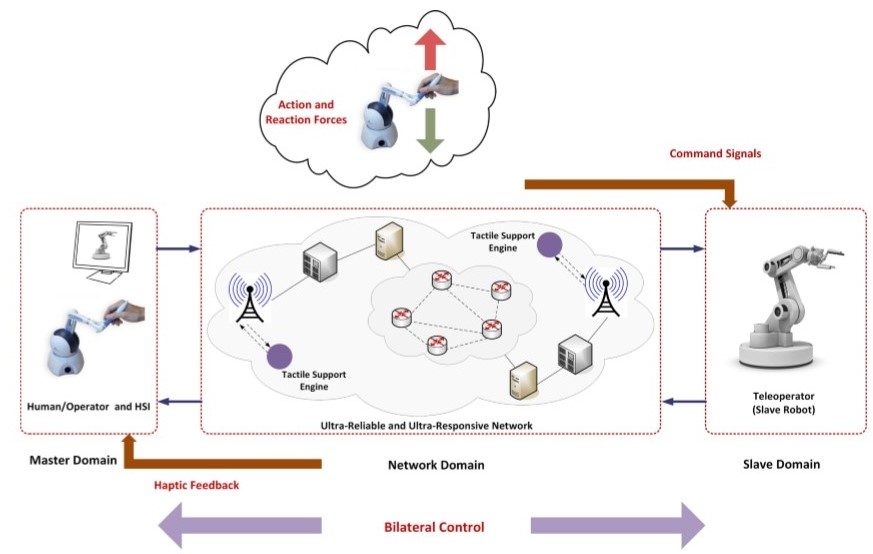
\includegraphics[scale=0.5]{imagem1.jpg}
\caption{Domínios na arquitetura da Internet Tátil ~\cite{Artigo1}}
\label{Rotulo}
\end{figure}
\setlength{\parindent}{0.5cm}
Como é visível na figura, entre a fonte e o recetor final, a arquitetura da Internet Tátil pode ser dividida em três sistemas diferentes: o domínio Mestre, o domínio da rede e o domínio submisso.

O domínio mestre consiste no utilizador humano, esteja ele a controlar diretamente um dispositivo com capacidade tátil ou a controlá-lo através de outra interface. Os equipamentos usados nesta fase fazem parte do sistema de interface humana (HSI em inglês) que é responsável por converter o input de dados gerados num pacote de dados táteis através de várias técnicas de codificação. Estes dispositivos táteis permitem ao utilizador tocar, sentir e manipular objetos em ambientes reais ou virtuais e controlar os equipamentos táteis no recetor final e podem simultaneamente enviar e receber dados de resposta e serem assim também parte do domínio submisso.

O sistema do domínio da rede providencia o meio para as comunicações em tempo real entre as fontes e os recetores. Idealmente, espera-se que o utilizador esteja totalmente imerso nos ambiente remotos com que interage. 

O recetor final, designado de domínio submisso, recebe as informações e comandos da fonte Mestre e reproduz as suas instruções. Este dispositivo final pode interagir com vários objetos no ambiente remoto em tempo real, reproduzindo assim as intenções que o utilizador comandou.


\subsection{Tempo de latência}
\setlength{\parindent}{0.5cm}
Exatamente porque a internet tátil irá suportar a disponibilização de serviços críticos para a sociedade e dia a dia do utilizador, esta implementação da rede terá que ter capacidade para um número gigantesco de utilizadores e aparelhos a comunicar entre si simultaneamente. Esta capacidade, devido à proliferação dos equipamentos tecnológicos pelos mais diversos meios e classes socias, terá que ser muito mais alargada que a capacidade da atual internet. Mais relevante que esta última preocupação, está o objetivo de criar uma rede capaz de ter uma latência (tempo de resposta) o mais baixo possível de forma a possibilitar que estes serviços críticos, como cirurgias, sejam efetivamente executados em tempo real. Esta questão do tempo de latência necessário para criar um sistema baseado em terminais hápticos, é um dos motivos pelo qual algumas das funcionalidades descritas nas potencialidades da internet tátil não estão implementadas na base da internet atual.

Em tarefas mais singelas do quotidiano, o tempo de latência mantem a sua importância, porque devido às interações táteis com o utilizador, se este notar atrasos no tempo de resposta poderá aperceber-se do Lag (como ocorre nos jogos que “travam” devido a más conexões à rede) e sofrer do chamado “CyberSickness” que pode causar náuseas e indisposições ao utilizador.  Além disso, o sistema não pode ter atrasos porque procuramos sistemas rápidos e fiáveis.

Retomando a questão do tempo de resposta (latência) baixa da rede que irá suportar a Internet Tátil, o maior desafio desta é alcançar um tempo de ida e volta de 1ms, sendo que por dia o sistema só pode falhar também por 1ms, de forma a ter uma disponibilidade perto dos 100\%. Percebendo que só com a latência de 1ms se instala a confiança necessária para uma interação tátil em tempo real, este é o desafio chave da Internet Tátil. Este tempo surge pelo tempo que o ser humano reage e sente o toque/perceção háptica.

\begin{figure}[!h]
\centering
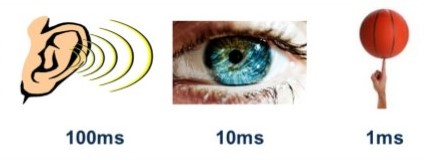
\includegraphics[scale=0.9]{imagem2.jpg}
\caption{Tempo de reação dos diferentes sentidos humanos ~\cite{Artigo2}}
\label{Rotulo}
\end{figure}

Considerando que as atuais ligações móveis e de internet 4G têm uma latência na ordem dos 20ms, um requerimento chave para as redes de quinta geração (5G) que irão ser base à Internet Tátil é terem este tempo de resposta inferior a 1ms.

\subsection{Dispositivos táteis}
\setlength{\parindent}{0.5cm}
Nesta estruturação da Internet Tátil, a introdução do toque é disponibilizada por dispositivos que permitam ao utilizador tocar, sentir e manipular objetos em ambientes reais ou virtuais. Curiosamente, estes equipamentos não são utopia nem o obstáculo da implementação da Internet Tátil. Alguns equipamentos com capacidade de receber/interpretar toque e induzi-lo já existem atualmente e alguns estão até disponíveis no mercado público. Contudo os custos de produção e manutenção, aliados à complexidade destes dispositivos têm que baixar consideravelmente para que exista uma adoção generalizada destes aparelhos e estes possam fazer parte dos mais diversos equipamentos do dia a dia e prestarem serviços nas mais diversas áreas da sociedade.

O design mais popular de um aparelho tátil é um sistema baseado num braço robótico com uma caneta anexada. O braço robótico rastreia a posição da caneta do utilizador e é capaz de exercer uma força na sua ponta, reproduzindo a escrita. Esta funcionalidade aliada a uma rede internet poderia permitir assinar contratos ou autorizações à distância ou numa aplicação adaptada, permitir que uma pessoa que não saiba escrever ou tenha dificuldades motoras nas mãos possa escrever usando apenas a voz.

Para compreender o alcance e visão da Internet Tátil é necessário um futuro desenvolvimento destes dispositivos táteis, principalmente aumentando a sua sensibilidade para responderem à demanda de serem usados em redes de tempo real e serviços críticos. Estes dispositivos serão a fonte e recetores finais da rede e estão descritos no gráfico da figura dois com a letra (1). Os restantes aspetos da figura serão descritos ao longo do presente documento.

\begin{figure}[!h]
\centering
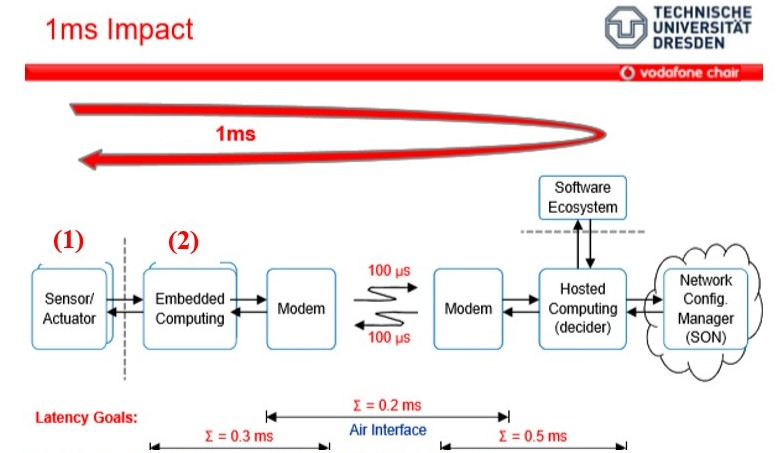
\includegraphics[scale=0.6]{imagem3.jpg}
\caption{Descriçâo das latências e estágios da implementação da Internet Tátil ~\cite{Gerhard}}
\label{Rotulo}
\end{figure}

\subsection{Codecs para informação tátil}
\setlength{\parindent}{0.5cm}
Com o surgimento de um novo tipo de informação a transmitir na rede, será ainda necessária uma nova linguagem de codecs, para codificar de forma standard em todos os dispositivos esta informação das comunicações táteis. Como os dispositivos usados como fonte/recetores de informação tátil geram uma grande quantidade de dados por segundo, têm vindo a ser investigadas diferentes técnicas para compreender os dados táteis gerados e explorar os limites da perceção tátil humana, ou seja, qual a quantidade de informação mínima necessária a transmitir para reproduzir um toque ou estímulo no utilizador sem que este perca a sensação de “realidade” naquilo que sente. Este é um fator importante, já que as redes têm em regra geral uma largura de banda limitada e portanto, os pacotes de dados gerados e recebidos devem ser o mais pequenos possíveis e sem que esta transmissão de informação tátil sobrecarregue a rede.

Um desafio fundamental no contexto da Internet Tátil é então o desenvolvimento de uma família de Codecs táteis padrão, semelhante aos atuais codecs ITU-T h.264 para vídeo e ISSO/IEC MPEG-4 para áudio. Englobando todo o tipo de informação tátil, esta linguagem de codecs será um fator fundamental para a implementação destas informações na rede e estaria implementada nos circuitos integrados que virão a fazer parte dos dispositivos com capacidade tátil falados anteriormente. Estas placas, representadas na figura um pelo numero (2), seriam capazes de codificar a informação vinda dos dispositivos fontes, codifica-la de forma padrão e envia-la para a rede. Num sentido oposto, a mesma placa seria capaz de receber dados da rede e descompactá-los para o dispositivo recetor final.


\subsection{Características da rede}
\setlength{\parindent}{0.5cm}
A necessidade de uma rede com estabilidade vem como um desafio natural para o desenvolvimento e implementação de aplicações como o controlo de objetos ou condução em tempo real, através dos serviços da internet tátil. Estas questões de instabilidade tornam-se importantes em sistemas de rede sem fios, onde atrasos com tempo imprevisível e variável podem levar a perdas de pacotes de informação e afetar fortemente a imersividade no ambiente remoto e no utilizador. Várias arquiteturas de controlo têm sido propostas nos últimos anos para estabilizar sistemas com interação háptica que sofrem de atrasos no tempo de resposta, tentando prever o movimento e ação do utilizador/fonte. No entanto, esta questão dos atrasos permanece amplamente sem solução.

Outra necessidade da rede que irá suportar a Internet Tátil será a sua disponibilidade. Nas redes de comunicações atuais, a disponibilidade da mesma é afetada por uma série de fatores externos, como a interferência incontrolável, diminuição da potência do sinal útil, falta de recursos, falhas de equipamento, localização do usuário, etc. Sendo a Internet Tátil usada para áreas-chave e serviços da sociedade requer, portanto, uma conectividade ultra fiável, sendo que os sistemas da rede devem estar disponíveis cerca de 100\% do tempo.

Esta disponibilidade será alcançada com um sistema onde se deseja que o tempo de interrupção do mesmo seja de 1ms por dia, estando no restante tempo sempre disponível e operacional, mantendo assim as perdas de pacotes na rede no mínimo possível.

Será ainda necessária uma reestruturação no modo como são implementados os protocolos de rede. Para reduzir as latências e garantir a segurança dos dados são necessárias várias otimizações em diferentes pilhas de protocolos abaixo da camada de IP. Cada fator que contribui para aumentar a latência deve ser otimizado para atingir os requisitos de resposta baixos da Internet Tátil e a camada física das futuras redes 5G devem ser projetadas para atender a este requisito crítico. 

\section{Conclusão}
\setlength{\parindent}{0.5cm}
Sendo a voz, vídeo, som e dados de informação os pacotes base que são partilhados pela internet atual, a Internet Tátil promete permitir em acréscimo a transmissão  de  comunicações  táteis,  levando  a  uma  mudança  de  paradigma  na  forma como interagimos com a rede e nela desempenhamos diferentes funções.

Por ser um tema sobre o qual ainda se fazem muitas especulações e pouca investigação e investimento, o desenvolvimento deste novo tipo de rede ainda está numa fase muito inicial e conceptual e julga-se que esteja apenas disponível e funcional só na próxima década.

\section{Bibliografia}
\bibliographystyle{unsrt}
\bibliography{Bibliografia}

\begin{thebibliography}{1}
\bibitem{Mischa Dohler}
Mischa Dohler,
\newblock{Kings College London}
\newblock{The Tactile Internet: Touch Me, Now You Can!}
\newblock{Disponível em: https://www.youtube.com/watch?v=ASphNkMOq-U}
\newblock{[Visualizado a 28 Setembro 2016]}

\bibitem{Martin Maier, Mahfuzulhoq Chowdhury, Bhaskar Prasad Rimal, Dung Pham Van}
Martin Maier, Mahfuzulhoq Chowdhury, Bhaskar Prasad Rimal, Dung Pham Van,
\newblock {The Tactile Internet: Vision, Recent Progress, and Open Challenges} (1965)
\newblock{Disponível em: http://ieeexplore.ieee.org/stamp/stamp.jsp?arnumber=7470948.}
\newblock{[Consultado a 3 de Outubro]}

\bibitem{Meryem Simsek, Adnan Aijaz, Mischa Dohler, Joachim Sachs, Gerhard Fettweis, IEEE}
Meryem Simsek, Adnan Aijaz, Mischa Dohler, Joachim Sachs, Gerhard Fettweis, IEEE
\newblock {5G-Enable Tactile Internet}
\newblock {Disponível em http://ieeexplore.ieee.org/stamp/stamp.jsp?arnumber=7403840}
\newblock{[Consultado a 3 de Outubro]}

\end{thebibliography}


\end{document}